% Figura - redes de migracao medica x fluxo de pacientes. src: 18_fig_physician_networks.py
\begin{figure}[t]
\centering
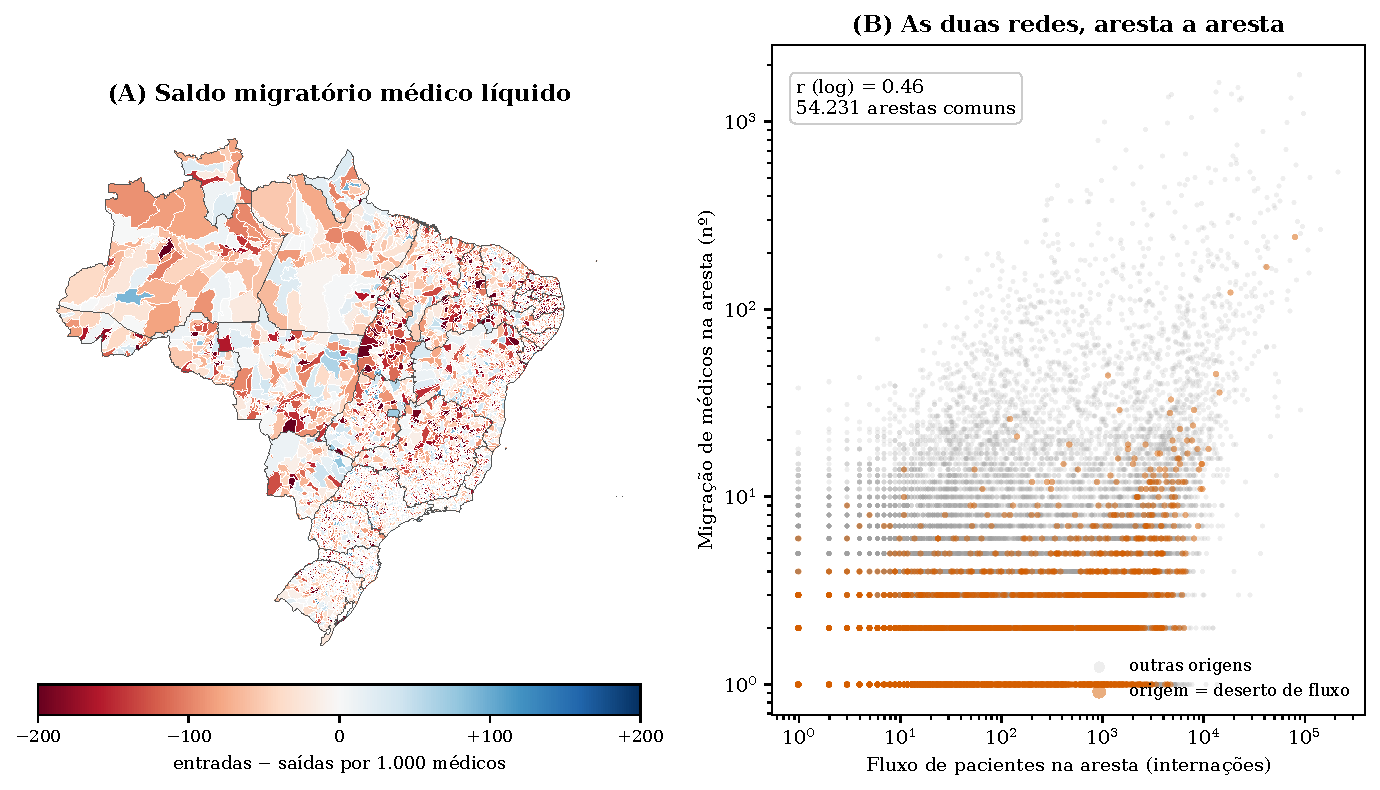
\includegraphics[width=\linewidth]{../04_figures/fig5_physician_networks.pdf}
\caption{\textbf{O deserto de fluxo tem dois lados.}
\textbf{(A)} Saldo migratório médico líquido por município (entradas $-$ saídas
por mil médicos, 2015--2023): em \textcolor[HTML]{B2182B}{vermelho}, municípios
que \emph{perdem} médicos; em \textcolor[HTML]{2166AC}{azul}, os poucos que
ganham. A maioria do território perde médicos para um punhado de hubs ---
geografia que espelha a do deserto de fluxo da Figura~\ref{fig:divergencia}.
\textbf{(B)} As duas redes município$\rightarrow$município, aresta a aresta:
fluxo de pacientes (eixo horizontal) contra migração de médicos (vertical), em
escala log. Os pesos são moderadamente correlacionados ($r=0{,}46$ em log, sobre
\valNetEdges{} pares comuns) --- médicos e pacientes deixam os mesmos lugares por
corredores parecidos ---, mas a coincidência não é exata: as arestas que partem
de desertos de fluxo (\textcolor[HTML]{D55E00}{laranja}) espalham-se, e o
principal destino dos médicos coincide com o dos pacientes em apenas \valTophubFO\% desses
municípios (Tabela~\ref{tab:medicos} e texto). Fonte: CNES-PF, SIH/DATASUS, IBGE.}
\label{fig:redes_medicas}
\end{figure}
